% !TEX root = root.tex
\chapter{Introduction}
\chaptermark{Introduction}

\section{Overview and Significance}

\section{Background}

\subsection{Rheology}

\subsubsection{Fundamentals}

Hooke's Law describes a solid as an idealized spring. A small deformation requires an applied force. The larger the deformation, the larger the requisite force, but the force in no way depends on the \emph{rate} of the deformation: fast and slow cost the same. A viscous liquid, as described by Newton's laws, behaves in a complementary way: it resists a small strain with a force proportional to the rate of strain but independent of the magnitude of that strain.

Real materials deviate from these simple pictures in two ways. First, if the force or deformation is large, the relationship between the applied stress and the strain (or, for liquids, strain rate) becomes more complicated than simple proportionality; the response is nonlinear. Second, even if the forces and deformations are small, some materials display both solidlike and liquidlike characteristics. For example, many materials respond elastically on short time scales but flow over long time scales. This temporal behavior reflects a spectrum of relaxation times that is dictated by the material's microstructural dynamics. Materials like these are viscoelastic.\cite{Ferry1980}

The theory of linear viscoelastic materials begins with a constitutive relation, a rheological equation of state relating stress $\sigma$ to strain $\gamma$. The equation states that changes in strain are linear. The shear modulus $G$ is a memory function representing the ratio of stress to strain through a given strain history.

\begin{equation}
  \label{eqn:linear-constituive}
  \sigma(t) = \int_{-\infty}^t G(t - t')\dot{\gamma}(t')\, dt'
\end{equation}

\noindent Let us apply this principle to a simple oscillatory strain, where a material is periodically deformed with some amplitude $\gamma_0$ at some frequency $\omega$.

\begin{equation}
  \gamma(t) = \gamma_0 \sin \omega t
\end{equation}

\noindent Eq. (\ref{eqn:linear-constituive}) gives

\begin{equation}
  \begin{aligned}
    \sigma(t) &= \int_0^\infty G(t - t') \gamma_0\,\omega \cos(\omega t')\, dt'\\
    &= \gamma_0\,\omega \int_0^\infty G(\Delta t) \cos[\omega (t - \Delta t)]\, d\Delta t\\
    &= \gamma_0 \left(\left[\omega \int_0^\infty G(\Delta t) \sin \omega \Delta t\, d\Delta t \right] \sin \omega t + \left[\omega \int_0^\infty G(\Delta t) \cos \omega \Delta t\, d\Delta t \right] \cos \omega t \right)
  \end{aligned}
\end{equation}

\noindent Because the bracketed factors depend only on $\omega$, we can define new functions $G'(\omega)$ and $G''(\omega)$, giving

\begin{equation}
  \sigma(t) = \gamma_0\, (G'(\omega) \sin \omega t + G''(\omega) \cos \omega t).
\end{equation}

\noindent The storage modulus $G'(\omega)$ gives the solidlike response, in phase with the oscillatory strain $\gamma(t)$, and the loss modulus $G''(\omega)$ gives the liquidlike response, 90$^\circ$ out of phase with the strain and hence in phase with the strain rate. They comprise the real and imaginary parts of the complex shear modulus, $G^*(\omega) = G'(\omega) + iG''(\omega)$, which is a fundamental linear response function and a quantity through which contact between theory and experiment is often achieved.

$G^*(\omega)$ provides a complete description of a material's linear shear response. Finite stresses and deformations can reveal rich, nonlinear responses, including a yield stress (some nonzero stress above which a solid no longer responds elastically but instead undergoes viscoplastic flow) or shear-thinning or -thickening (where the effective viscosity of the fluid decreases or increases with the applied strain rate).
\subsubsection{Measurement Techniques}

There is a large family of well-established techniques for measuring a material's frequency-dependent shear modulus $G^*(\omega)$. The stress--strain relationship can be probed in either direction, by applying a certain stress and measuring the resultant strain or by measuring the stress necessary to enforce a certain strain. For example, a creep experiment measures the strain in response to a sudden stress, whereas a stress relaxation experiment measures the stress following a sudden strain. Both of these are transient experiments, observing the material's response as a function of time after a sudden change. Oscillatory experiments provide complimentary information, applying a periodic stress or strain at some frequency $\omega$, qualitatively probing the same response as a transient experiment at time $t=1/\omega$. Oscillatory experiments are especially important for probing short-time scale or (high-frequency) behavior.

Shear rheology measurements, whether transient or oscillatory, strain-controlled or stress-controlled, can be performed in many different geometries. Important ones include simple shear flow between translated parallel plates or, equivalently and more commonly, between a rotating cone and plate; shear between rotating coaxial cylinders (Couette flow); flow inside a rectangular slit; and shear between two rotating parallel plates.

All of these are, of course, subject to limitations. In oscillatory experiments the inertia of the rotating tool can dominate the shear response of the sample at  high frequencies. And all experiments contend with the problem of slip, the possibility that the sample might lose mechanical contact with a bounding surface where its velocity was assumed to be zero with respect to the surface.

\subsection{Interfacial Rheology\label{sec:interfacial-rheology}}

Interfacial layers at the boundary between two fluids exhibit the same complex, non-Newtonian, and nonlinear behavior observed in bulk materials. The central experimental challenge in characterizing these interfaces is isolating the interfacial rheological response from the response of the surrounding fluids, as the flows at the interface and the bulk fluids are intimately coupled\cite{Fuller2011}. The relative contributions of surface and bulk forces on a rheological probe is captured by the Boussinesq number\cite{Derkach2009}

\begin{equation}
  \label{eqn:simple-bo}
  \text{Bo} = \frac{\eta_s}{l(\eta_1 + \eta_2)}
\end{equation}

\noindent where $\eta_s$ is the surface viscosity and $\eta_{1,2}$ are the bulk viscosities of the fluids above and below. In many experiments, these viscosities of the fluids are matched ($\eta_1 + \eta_2 = 2\eta_2$) or else one is air and can be neglected ($\eta_1 + \eta_2 = \eta_2$). Surface viscosity and bulk viscosity differ by a dimension of a length, and a length scale $l$ is introduced. The definition of $l$ depends on the particulars of the geometry of the technique. Heuristically, $l$ is sometimes presented as the ratio of the interfacial surface area subtended by the probe to its perimeter of contact with the interface. But this picture of $l$ does not hold, even qualitatively, for some geometries\cite{Levine2004}.

For $Bo \gg 1$, interfacial rheology dominates the force on the rheological probe. For $Bo \ll 1$, forces from the bulk fluid dominate. Thus, a well designed technique maximizes Bo by minimizing $l$. And, unless the contribution from the bulk is negligible, the technique must be have an accompanying theory for separating the interfacial and bulk contributions.


Eq. (\ref{eqn:simple-bo}) applies to a simple viscous interface, but Bo can be generalized for viscoelastic interfaces\cite{Fuller2012}:

\begin{equation}
  \text{Bo}(\omega) = \left|\frac{G_s''(\omega) - i G_s'(\omega)}{\omega l(\eta_1 + \eta_2)}\right|
\end{equation}


Experimental techniques tackle the challenge of isolating the interfacial response in very different ways. One is a bicone or disk, centered at the interface and operated like a traditional rotating-tool rheometer. The torque on the disks is separated into the components using methods of continuum mechanics\cite{Derkach2009}, initially worked out by Boussinesq himself\cite{Boussinesq1913} and later refined\cite{Oh1978}. The tool makes a full circular patch in the interface and couples strongly to bulk flows, diminishing its sensitivity to the interfacial rheology. This is quantified by the Boussinesq number: the length scale $l$ is related to the radius of the tool, diminishing Bo for given viscosities $\eta$, $\eta_2,$ $\eta_s$.

A newer technique improves sensitivity by replacing the bicone with a double wall-ring geometry\cite{Vandebril2010}. The open center of the ring diminishes coupling to bulk flows, and the important scale $l$ becomes the thin width of the ring rather than its radius.

Other techniques rely on millimeter- to micron-scale probes manipulated by applied optical or magnetic forces. The most popular of these, dubbed the Interfacial Shear Rheometer (ISR), moves a needle pinned to the interface by capillary forces, through oscillatory translations along its axis\cite{Brooks1999} with a magnetic force within a channel to create the equivalent of a parallel plate rheometer. Others use magnetic force to rotate a thin rod\cite{Lee2009,Lee2010} or a disk\cite{Zell2014} or in the plane of the interface. In this work, we employ a rotating needle.

%On the Superficial... http://archive.org/stream/scientificpapers03rayliala/scientificpapers03rayliala_djvu.txt

\section{Microrheology}

Microrheology relates the motion of colloidal particles to the rheology of the surrounding medium. Often, the motion is thermally-driven Brownian fluctuation (``passive microrheology'') but in recent years the field has come to encompass ``active microrheology'', where colloids driven by optical or magnetic forces can probe stiffer materials and larger deformations, extending into the regime of nonlinear response.

When probes are confined to an interface, the technique is sensitive interfacial viscosities as small as 1 nPa$\cdot$s$\cdot$m, well below the range of traditional techniques, and can characterize shear response over a wide of range of frequencies ($10^{-2}$--$10^4$ Hz) \cite{Waigh2005}.

\subsection{Fundamentals}

The fundamental relation of microrheology is the Generalized Stokes--Einstein Equation. The ``Einstein'' part relates a statistical characterization of probe motion (probe mean-squared displacement $\langle \Delta r^2 \rangle$) to a deterministic property (mobility $M$), which the ``Stokes'' part then relates to the rheological properties of the material. For a probe of radius $a$ diffusing in a viscous medium, the Stokes--Einstein relation gives

\begin{equation}
\langle \Delta r^2(t) = \frac{N k_B T}{6\pi\eta a}
\end{equation}

for the $N$-dimensional mean-squared displacement. The Generalized Stokes--Einstein posits a frequency-dependent mobility $M(\omega)$ or, equivalently, hydrodynamic drag $\zeta(\omega)$. As originally derived\cite{Mason1995,Mason2000}, and later reviewed in detail\cite{Squires2010}, the generalized form can be derived from the generalized Langevin equation, an equation of motion incorporating a random thermal force $f_R$ and a frequency-dependent hydrodynamic drag $\zeta$.

\begin{equation}
  m\dot{v}(t) = f_R(t) - \int_0^t\zeta(t-t')v(t')\,dt'
\end{equation}

\noindent Because the random force $f_R$ is stochastic, $v(t)$ must be treated statistically. Temperature $T$ is introduced through the equipartition theorem, and the uncorrelated nature of $f_R$ causes it to drop out. At low Reynolds number, inertia is negligible compared to hydrodynamic forces, and so mass $m$ also drops out. The result is the Generalized Stokes--Einstein equation, relating the complex frequency-dependent shear modulus $G^*(\omega)$ to the unilateral Fourier transform observed $N$-dimensional mean-squared displacement:

\begin{equation}
G^*(\omega)=\frac{N k_B T}{3 \pi i\omega\mathcal{F}_u\left\{\langle \Delta r^2 (t)\rangle\right\}}
\end{equation}


\noindent Alternatively, can be written in terms of the complex shear compliance $J(t)$,\cite{Squires2010} which is related to shear relaxation modulus $G(t)$ through $\int J(t)G(t) = 1$.\cite{Ferry1980}

\begin{equation}
J(t) = \frac{Nk_B T}{3\pi a \langle r^2(t) \rangle}
\end{equation}

\noindent This expression has the advantage of being algebraic, and thus does not require the data to undergo a numerical integral transform\cite{Larsen2008}.

\subsection{\label{sec:interfacial-microrheology}Interfacial Microrheology}

As described in Section \ref{sec:interfacial-rheology}, experimental techniques for measuring interfacial rheology should maximize their sensitivity to the interface relative to the bulk (i.e., maximize Bo), and they should include a procedure for separating the interfacial and bulk contributions. Interfacial microrheology faces the same challenge. Because microrheological probes are typically micron-scale, the geometrical length scale $l$ is small, and sensitivity to the interface is high relative to the macrorheology techniques. The sensitivity allows microrheology to characterize interfaces with much smaller interfacial viscosity. Nonetheless, coupling to the bulk at some point becomes appreciable; the problem of separating the contributions of bulk and interface must still be addressed.

\subsection{Translational drag on a sphere at an interface}

For viscous layers, the translational drag $\zeta$ on a circular inclusion in a membrane was first determined by Saffman and Delbruck, who showed that a physically meaningful description of interfacial Stokes drag must incorporate coupling to the surrounding phase(s)\cite{Saffman1975}.

\begin{equation}
\frac{1}{\zeta} = \frac{1}{4\pi\eta_s}\left(\log(\text{Bo}) - \gamma\right)
\end{equation}

\noindent where $\text{Bo}=\eta_s/[(\eta_1 + \eta_2)\, a]$ for a sphere of radius $a$ and $\gamma$ is Euler's constant (0.5772...). The Saffman--Delbruck expression is invalid at low Bo. When $\log(\text{Bo}) < \gamma$, it gives $D < 0$, which is of course unphysical. A more general form was worked out by Hughes\cite{Hughes1982} and reduced to a nice closed form by Petrov and Schwille\cite{Petrov2008}:

\begin{equation}
\begin{aligned}
\displaystyle\frac{1}{\zeta} = &\frac{1}{4\pi\eta_s}\\
    &\times\ \log(2/\epsilon) - \gamma + 4\epsilon/\pi - (\epsilon^2/2)\log(2/\epsilon)\\
&\times\ \left[1 - (\epsilon^2/\pi)\log(2/\epsilon) + c_1\epsilon^{b_1}/(1 + c_2\epsilon^{b_2})\right]^{-1}
\end{aligned}
\end{equation}

\noindent where $\epsilon$ is simply inverse Boussinesq number $1/\text{Bo}$ and the numerically-determined constants are $c_1 = 0.73761$, $b_1 = 2.74819$, $c_2 = 0.52119$ and $b_2= 0.61465$.

    \begin{figure}
    \centering
    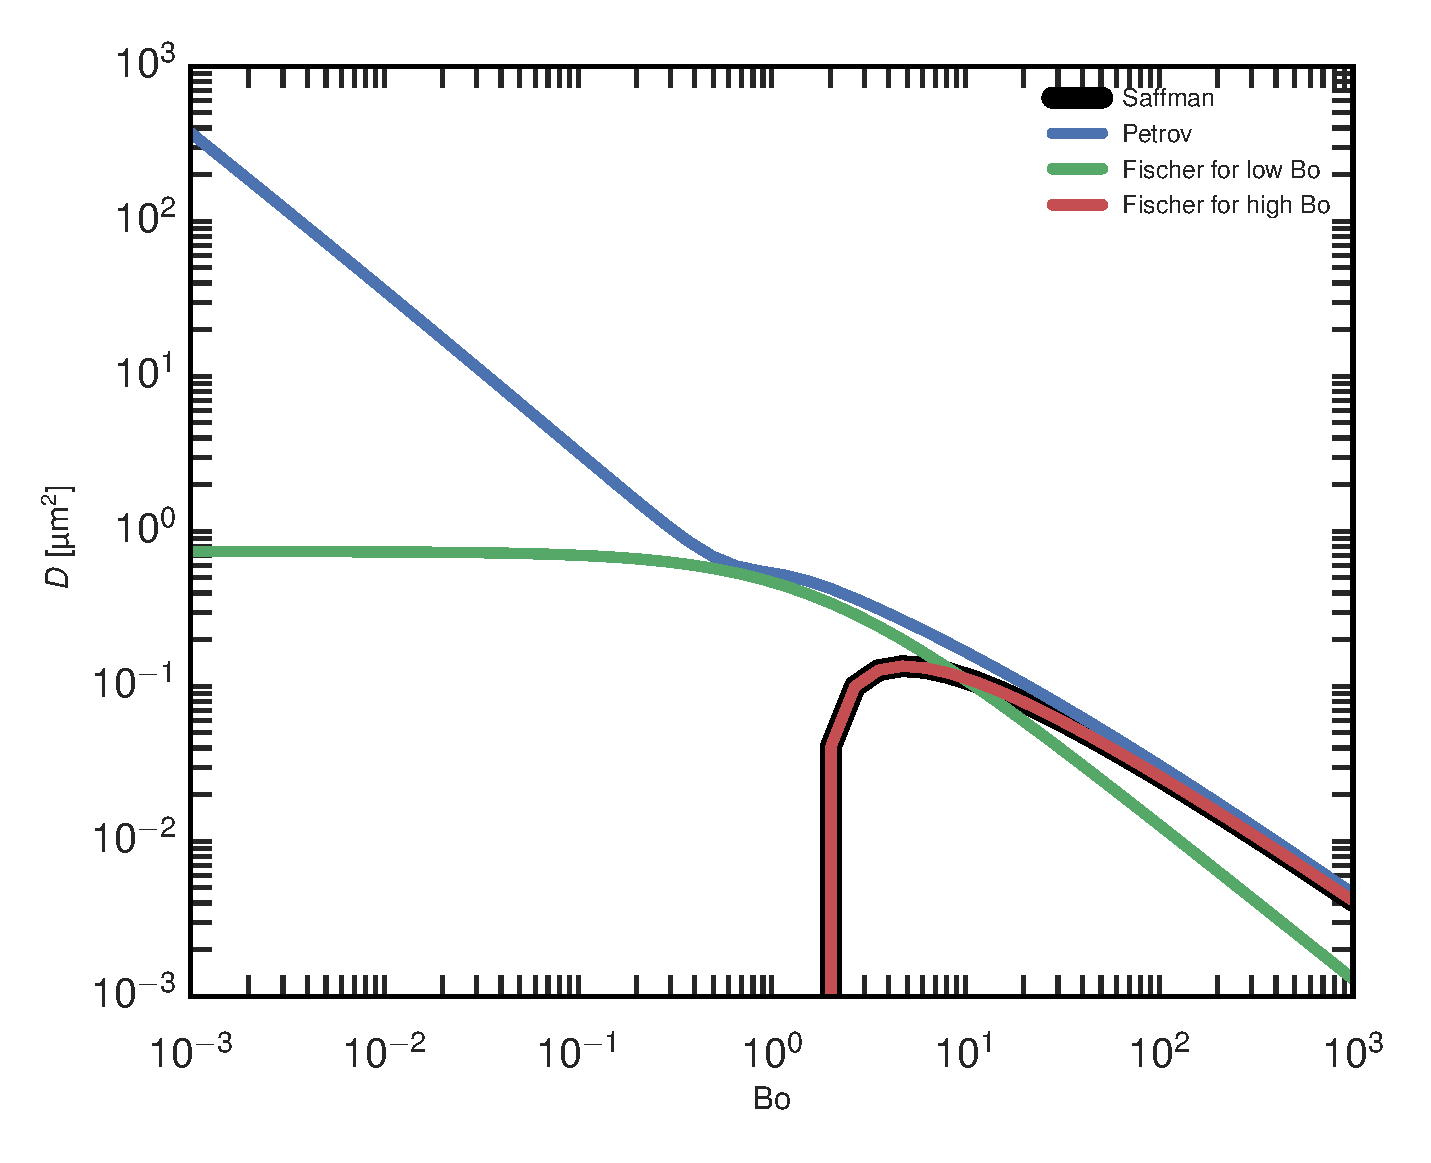
\includegraphics[width=\columnwidth]{introduction/drag-models}
    \caption{\label{fig:drag-models}A comparison of models for the translation drag on a membrane inclusion. This figure is closely modeled after one by Samaniuk\cite{Samaniuk2014}, simply comparing more models.}
    \end{figure}

A more elaborate model, the Fischer model, accounts for the contact angle $\theta$ of a spherical inclusion and the effect of Marangoni forces---surface tension gradients produced by concentration gradients across the interface. At Bo $\ll 1$, the Fischer model gives the translation drag coefficient $\zeta$ as an expansion in Bo \cite{Fischer2006}

\begin{equation}
  \label{eqn:fischer-low-bo}
  \zeta = \eta a (k^{(0)} + \text{Bo}\, k^{(1)} + o(\text{Bo}^2))
\end{equation}

\noindent with coefficients (within 3\% accuracy)

\begin{align}
  k^{(0)} &\approx 6\pi\sqrt{\tanh[32(d/a + 2)/9\pi^2}\\
  k^{(1)} &\approx -4\ln\left(\frac{2}{\pi}\tan^{-1}\left(\frac{d + 2a}{3a}\right)\right)
\end{align}

where $d$ is the distance from the apex of the particle to the level of the interface; $d$ is defined to be positive when the particle is fully submerged and negative when the particle is embedded. Assuming gravitational and capillary effects are negligible, so that the surface remains flat in the vicinity of the sphere, $d$ can be expressed in terms of the contact angle $\theta_c$ as $d=a(\cos \theta_c - 1)$.

In the opposite limit, Bo $\gg 1$,

\begin{equation}
  \label{eqn:fischer-high-bo}
  \zeta = \eta a \left(\frac{4\pi\text{Bo}}{\ln(\text{Bo}\, a/a_s) - \gamma}\right).
\end{equation}

\noindent where $a_s$ is the cross-section of the particle at the interface and $\gamma$ is the Euler number. In this limit, $\eta_s$ is negligible and thus not measurable, and so it might seem to be of little use. But when Eq. (\ref{eqn:fischer-low-bo}) and Eq. (\ref{eqn:fischer-high-bo}) are plotted together in Figure \ref{fig:drag-models}, boldly extended through and beyond the domains of mathematical validity, including through $0.1 \ll \text{Bo} \ll 10$ where neither is valid, we see agreement at least up to the order of magnitude throughout. As has been previously observed\cite{Samaniuk2014}, this agreement may explain the surprising agreement between different theoretical approaches\cite{Maestro2011}.


\subsection{Rotational drag on a rod at an interface}

As with the diffusivity of the spheres, the mobility of the
rotating wires depends on both the interfacial and subphase properties. The relative importance of these contributions can be parametrized by the Boussinesq number. For a highly anisotropic object, such as a wire-shaped colloid, it has been theorized\cite{Levine2004} that the characteristic length scale entering the Boussinesq number is the wire length $L$ and that the rotation drag is independent of the object's aspect ratio.

\begin{equation}
\text{Bo} = \frac{\eta_s}{L(\eta_1 + \eta_2)}
\end{equation}

\noindent At high Bo, the theory predicts\cite{Levine2004} rotational drag coefficient $\zeta_r \rightarrow 1.48\eta_s L^2$; at low Bo, $\zeta_r \rightarrow 0.50\eta L^3$. Measurements on Ni nanowires within viscous protein layers comparing the drag for translation parallel to the wire axis $\zeta_\parallel$
 with $\zeta_r$ indicate that the results of this theory accurately predict $\zeta_\parallel/\zeta_r$,\cite{Lee2010} and we use their theory to analyze the wire rotation.

\section{Protein Layers}

Under many circumstances proteins adsorb at air--water interfaces\cite{Mobius1998}. Like small-molecule surfactants, interfacial proteins can stabilize emulsions and foams through reducing surface tension or by forming coalescence-arresting viscoelastic skins on the surfaces of drops and bubbles\cite{SaintJalmes2005,McClements2004}. The surfactant-like character of proteins is crucial to many current and developing technologies, particularly those related to the food, biomedical, and pharmaceutical industries. In addition, interfacial protein layers perform physiological functions in vivo\cite{Alonso2005,Proctor2005}. Proteins at fluid interfaces typically change their conformations, i.e., denature, in a way that reduces their free energy by bringing to the surface the hydrophobic parts that are normally folded inside the structure, shielded from the surrounding water. This unfolding can make adsorption irreversible, and hence equilibrium between interfacial proteins and those in the bulk solution is lost. At sufficient concentration, interfacial protein layers can acquire pronounced viscoelastic behavior \cite{Mobius1998,Graham1978,Bos2001,Murray2011a} that has been attributed either to the formation of a gel-like network through intermolecular bonding\cite{Bos2001,Murray2011a,Bantchev2003, Roberts2005,Freer2004,Petkov2000,Wijmans1998} or to kinetic arrest due to steric jamming\cite{Wierenga2006,Cicuta2005,Cicuta2003,Cicuta2007}. In many cases this elasticity is key to protein layers� utility. For example, mechanically strong interfacial layers resist tangential stresses from flow in the adjoining liquids, preventing rupture and coalescence of droplets and bubbles. Further, the properties of protein layers can provide a unique perspective on issues of protein denaturation, protein-protein interactions, and the gel transition.

Due to the importance of the mechanical properties of protein layers, numerous experiments have sought to characterize their interfacial shear rheology\cite{Proctor2005,Bos2001,Bantchev2003,Roberts2005,Freer2004,Petkov2000,Wierenga2006,Cicuta2005,Cicuta2003,Cicuta2007,Miller1996,Murray1998,Jones2002,Blomqvist2004,Martin2005,Erni2003,Freer2004,Vessely2005,Ariola2006,Kragel2008}. These studies have had to contend with the significant technical difficulties inherent to interfacial rheology, as addressed in the previous section. Additionally, protein layers are fragile, molecularly thin, and spatially heterogeneous with properties that evolve with time. These features complicate traditional interfacial rheometry measurements and often make results difficult to interpret. Interfacial microrheology, introduced in Section \ref{sec:interfacial-microrheology}, is ideally suited to address these difficulties.

Previous work by our group on the microrheology of the protein $\beta$-lactoglobulin layers\cite{Lee2010} supports the gelation picture, in which proteins associate through intermolecular disulfide bonds. My work applied similar techniques to layers of lysozyme and Staphylococcal nuclease (SNase) in an effort to understand better those aspects of the viscoelastic transition in protein layers that are universal and those that are system specific. Lysozyme, $\beta$-lactoglobulin, and SNase are single-chain globular proteins that have been widely studied for decades. They are stable in bulk solution (i.e., they do not rapidly aggregate) but they readily adsorb to the air--water interface. For the SNase study in particular, we isolated the role of protein unfolding in evolution of the layer's mechanical response. We studied wild-type SNase---the protein as it is found in nature---and an engineered variant that shared almost the same chemical composition but had a completely disordered, unfolded structure.

The studies included passive measurements, which tracked the Brownian motion of spherical colloids at the interface, and active measurements in which the rotational motion of magnetic nanowires at the interface was employed to infer layer rheology.

\section{Bacterial Biofilms}

At a fluid interface, bacteria form a biofilm---a film of bacteria and its products---and this film can alter the mechanical properties of the interface. Specifically, the film comprises adherent cells in a complex matrix of extracellular polymeric substances including polysaccharides and surfactants secreted by the bacteria\cite{Watnick2000}. These films thus resemble from a physical-sciences perspective a disordered colloidal suspension with added polymer. Composite materials of this type can be expected to possess mechanical properties characteristic of disordered and glassy complex fluids and soft solids. Indeed, research has shown how complex fluids, such as polymers mixed with colloids, can form soft glassy phases under a range of conditions\cite{Cipelletti2005,Mewis2009,Stokes2008,Bandyopadhyay2005}. These phases are distinguished by novel mechanical properties including thixotropic (shear-thinning) response to stress and anomalous low-frequency viscoelastic moduli \cite{Cipelletti2005,Mewis2009,Stokes2008,Bandyopadhyay2005}. In addition, these disordered materials are typically out of equilibrium, and their mechanical behavior can evolve perpetually, a process known as aging\cite{Cipelletti2005,Bandyopadhyay2005}. Many of these properties are associated with metastable heterogeneous structure in these mixed systems and strong mechanical coupling between components. Theory exploring the dynamics and aging of soft glassy systems has emphasized their apparent universality\cite{Sollich1998,Fielding2000,Coussot2007,Fielding2009}. Recent research has also identified characteristics shared by biofilms formed on solid substrates and such glassy soft solids\cite{Rogers2008,Hohne2009,Wilking2011a,Pavlovsky2013}.

Bacterial biofilms form where spilled oil creates an interface between oil and ocean water, and much has been done to increase the speed and ability of the bacteria to degrade pollutant hydrocarbons\cite{Abbasnezhad2011, Warr2013}. Additionally, the mechanical behavior of this interfacial layer is thought directly to influence petroleum extraction. Stiff films can limit the ability of oil droplets to pass through narrow pores and channels, competing with the reductions in interfacial tension and viscosity that promote recovery. On the other hand, the formation of stiff interfacial films has also been advanced as a mechanism for the clogging of highly permeable regions of reservoirs that aids in enhanced recovery\cite{Jenneman2013}. Despite this significance, few studies have reported on the mechanical properties of bacterial films at oil-water interfaces. The in-plane mechanical behavior of an interfacial film is characterized by its response to two modes of deformation: its shear modulus, which describes the response to area-conserving deformations, and its dilational modulus, which describes the response to changes in area. Previous research on the mechanical behavior of bacterial films at an oil-water interface has focused exclusively on their response to dilational stress\cite{Kang2008,Kang2008a}, leaving key aspects related to their shear rheology unexplored.

Such information is crucial for understanding the films� mechanical response both from a fundamental perspective and in the context of enhanced oil recovery. For example, the resistance to tangential stresses provided by the shear modulus can dictate the stability of an interfacial layer to rupture\cite{Edwards1991}. In addition, analysis of shear rheology can give access to interaction forces in an interfacial layer, shedding light on the mechanisms dictating the strength and compliance of the films\cite{Miller1996}. Chapter \ref{chap:bacteria} describes experiments that addressed these important issues by investigating the linear shear rheology of model bacterial films at an oil-water interface.